\documentclass{article}

%%%%%%% PACKAGES %%%%%%%%
\usepackage[utf8]{inputenc}
\usepackage[margin=2cm]{geometry}
\usepackage{blindtext}
\usepackage{setspace}
\usepackage{graphicx}
\usepackage{hyperref}
\usepackage{notoccite} %citation number ordering
\usepackage{lscape} %landscape table
\usepackage{caption} %add a newline in the table caption
\usepackage{subfig}
\usepackage{float}

\usepackage[
    backend=biber,  %references format (IEEE)
    style=ieee,
    sorting=none
]{biblatex}
\addbibresource{references.bib} %rename this to your own bibliography
\onehalfspace   % 1.5 line spacing

\title{\huge{\textbf{Global Warming and Climate Change}}\\
    \LARGE{Renewable Energy Assignment 1}}
\author{Ali Asghar Yousuf - ay06993}
\date{\today}

\begin{document}
\pagenumbering{roman} % Start roman numbering
\clearpage\maketitle
\thispagestyle{empty}
\begin{center}
    \begin{figure}[h]
        \centering
        \includegraphics[width=10cm]{hu_logo.png}
        %\caption{Your caption here}
        \label{fig:logo}
    \end{figure}
    \large{ENER 104 Renewable Energy \\
        Mohamed Elsayed Orabi Mustafa}
\end{center}
\newpage
\setcounter{page}{1}
\tableofcontents

\newpage
\pagenumbering{arabic} % Start roman numbering

%%% CONTENT HERE %%%%
\section{Introduction}
This report will discuss the effects of global warming and climate change on
the environment and the world. It will also discuss the causes of global
warming and climate change and how they can be prevented. The report will also
discuss the relevance of global warming and climate change to Pakistan, and how
the country can prevent global warming and climate change.

Global warming is the increase in the average temperature of the Earth's
surface. This is caused by the greenhouse effect, which is the process by which
radiation from a planet's atmosphere warms the planet's surface to a
temperature above what it would be without this atmosphere. Climate change is a
change in the statistical distribution of weather patterns when that change
lasts for an extended period of time. Climate change may refer to a change in
average weather conditions, or in the time variation of weather around
longer-term average conditions.

\section{Causes of Global Warming and Climate Change}

\subsection{Greenhouse Gases}
Greenhouse gases are gases that absorb and emit radiant energy within the
thermal infrared range. Greenhouse gases cause the greenhouse effect on
planets. The primary greenhouse gases in Earth's atmosphere are water vapor,
carbon dioxide, methane, nitrous oxide, and ozone. Without greenhouse gases,
the average temperature of Earth's surface would be about $-18^{\circ}C$
(0$^{\circ}F$), rather than the present average of $15^{\circ}C$
(59$^{\circ}F$). The atmospheres of Venus, Mars and Titan (largest moon of
Saturn and second largest in our solar system) also contain greenhouse gases.
Human activities since the beginning of the Industrial Revolution (around 1750)
have produced a 40\% increase in the concentration of carbon dioxide in the
atmosphere, from 280 ppm in 1750 to 400 ppm in 2015 \cite{US_EPA}. This
increase has occurred despite the uptake of more than half of the emissions by
various natural "sinks" involved in the carbon cycle. The vast majority of
anthropogenic carbon dioxide emissions come from combustion of fossil fuels,
principally coal, oil, and natural gas, with additional contributions coming
from deforestation, changes in land use, soil erosion and agricultural
practices, and some industrial processes such as cement manufacturing.

\subsection{Carbon Dioxide}
Carbon dioxide is the primary greenhouse gas that is contributing to recent
climate change. Carbon dioxide is naturally present in the atmosphere as part
of the Earth's carbon cycle. Human activities are altering the carbon cycle
both by adding more $CO_2$ to the atmosphere and by influencing the ability of
natural sinks, like forests, to remove $CO_2$ from the atmosphere. While $CO_2$
emissions come from a variety of natural sources, human-related emissions are
responsible for the increase that has occurred in the atmosphere since the
industrial revolution. The main human activity that emits $CO_2$ is the
combustion of fossil fuels (coal, natural gas, and oil) for energy and
transportation, although certain industrial processes and land-use changes also
emit $CO_2$.

\subsection{Methane}
Methane ($CH_4$) is a hydrocarbon that is a primary component of natural gas.
Methane is emitted during the production and transport of coal, natural gas,
and oil. Methane emissions also result from livestock and other agricultural
practices and by the decay of organic waste in municipal solid waste landfills.
Methane is also emitted from multiple sources within the transportation sector,
including emissions from the refinement and distribution of petroleum products,
as well as from the incomplete combustion of fuels.

\subsection{Nitrous Oxide}
Nitrous oxide ($N_2O$) is a powerful greenhouse gas that is emitted from
agricultural and industrial activities, as well as during combustion of fossil
fuels and solid waste. Nitrous oxide emissions occur naturally through
microbial processes in soils and the ocean, as well as through human activities
involving fertilizer use, fossil fuel combustion, nitric acid production, and
biomass burning.

\subsection{Fluorinated Gases}
Hydrofluorocarbons, perfluorocarbons, and sulfur hexafluoride are synthetic,
powerful greenhouse gases that are emitted from a variety of industrial
processes. Fluorinated gases are sometimes used as substitutes for ozone
depleting substances in various applications, such as refrigeration and
air-conditioning, aerosols, foams, and fire suppression. These gases are
typically emitted in smaller quantities, but because they are potent greenhouse
gases, they are sometimes referred to as High Global Warming Potential gases
(``High GWP gases'').

\section{Effects of Global Warming and Climate Change}
\subsection{Rising Sea Levels}
Global sea level has risen by about 8 inches in the last century. The rate in
the last two decades, however, is nearly double that of the last century and is
accelerating slightly every year \cite{Lindsey}. As it warms, the water in the
oceans expands. Warmer water also causes the ice on land to melt and flow into
the oceans. The melting of the polar ice caps and glaciers due to global
warming will lead to a rise in sea level. This will lead to flooding of low
lying coastal areas and also cities. The flooding in these densely populated
areas would lead to massive property losses and loss of life. In many cases,
the effects of flooding can be devastating, and they can leave a lasting impact
on the affected areas. Some of the most common effects of flooding are property
damage, loss of agricultural lands, loss of lives, and diseases.

\subsection{Wildfires}
Wildfires are becoming more frequent and intense due to climate change and
other factors. Wildfires are uncontrolled fires that burn forests and other
wildlands, sometimes spreading to residential areas. Wildfires have occurred
naturally ever since the first plants colonized the Earth, about 400 million
years ago. Wildfires can be caused by natural factors such as lightning, but
also by human activities, the most common of which is arson. Wildfires can
cause extensive damage, both to property and human life, but they also have
various beneficial effects on wilderness areas. They help to clear dead brush
and trees from forests, allowing new growth to flourish. They also help to
return nutrients to the soil, which helps to promote the growth of new plants.
Wildfires can also help to control insect populations, which can be harmful to
trees and other plants.

\subsection{Droughts}
As flooding becomes more frequent and intense due to climate change, droughts
are becoming more frequent and intense as well. Droughts are periods of time
when there is little or no rainfall. Droughts can be caused by natural factors
such as lack of rainfall, but also by human activities, such as overuse of
water resources. Droughts can disrupt the water supply, which can lead to water
shortages and rationing. Droughts can also lead to crop failures and famine,
which can lead to mass migration and conflict.

\subsection{Heat Waves}
Heat waves are periods of time when the temperature is unusually high. Heat
waves can cause heat-related illnesses, such as heat stroke, heat exhaustion
and in extreme cases, death. Heat waves also result in increased energy demand,
which can lead to power outages and blackouts.

Global warming and climate change can also lead to other extreme weather
events, such as hurricanes, tornadoes, and floods. These events are common in
many parts of the world, and they cause extensive damage to property and
infrastructure every year.

\subsection{Other Effects}
Global warming and climate change can also lead to other effects, such as
increased ocean acidity, which can lead to the death of coral reefs and other
marine life. Global warming and climate change can also lead to the spread of
diseases, such as malaria and dengue fever, which are spread by mosquitoes.
Global warming has also increased the energy demand worldwide due to increased
use of air conditioning and refrigeration, which has led to increased use of
fossil fuels, which has led to increased greenhouse gas emissions, which has
led to increased global warming and climate change.

\section{Prevention of Global Warming and Climate Change}
\begin{figure}[H]
	\centering
	\subfloat[Annual $CO_2$ Emissions]{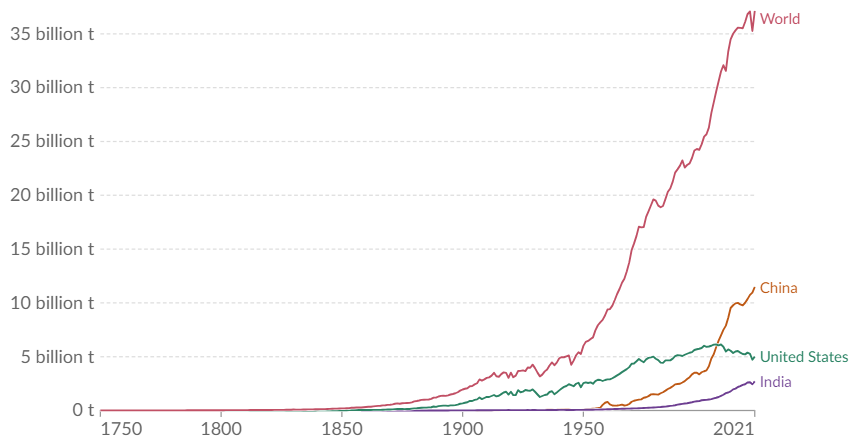
\includegraphics[width=0.45\columnwidth]{annual.png}}
	\qquad
	\subfloat[Annual Changes in Renewable Energy generation]{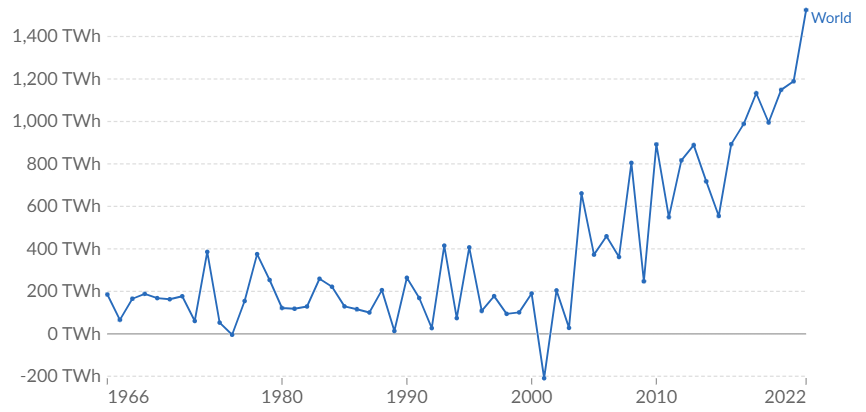
\includegraphics[width=0.45\columnwidth]{renewable.png}}
	\label{fig:Comparison}
\end{figure}

While we see an increasing trend in global $CO_2$ emissions, we also see a 
glimpse of hope as the renewable energy generation is also increasing. This
shows that we are moving in the right direction, but we need to do more to
prevent global warming and climate change.
\subsection{Renewable Energy}
Renewable energy is energy that is collected from renewable resources, which
are naturally replenished on a human timescale, such as sunlight, wind, rain,
tides, waves, and geothermal heat. Renewable energy often provides energy in
four important areas: electricity generation, air and water heating/cooling,
transportation, and rural (off-grid) energy services. Based on REN21's 2017
report, renewables contributed 19.3\% to humans' global energy consumption and
23.5\% to their generation of electricity in 2015 and 2016, respectively
\cite{REN21}.

\subsection{Energy Efficiency}
Energy efficiency is the goal to reduce the amount of energy required to
provide products and services. For example, insulating a home allows a building
to use less heating and cooling energy to achieve and maintain a comfortable
temperature. Installing LED lighting, fluorescent lighting, or natural skylight
windows reduces the amount of energy required to attain the same level of
illumination compared to using traditional incandescent light bulbs. Improving
energy efficiency reduces energy cost per unit of service, and can reduce
greenhouse gas emissions depending on how electricity is generated. Energy
efficiency and renewable energy are said to be the twin pillars of sustainable
energy policy and are high priorities in the sustainable energy hierarchy. In
many countries energy efficiency is also seen to have a national security
benefit because it can be used to reduce the level of energy imports from
foreign countries and may slow down the rate at which domestic energy resources
are depleted.

% Where Does Pakistan Stand in Terms of Global Warming Contributors?
\section{Relevance to Pakistan}
\subsection{Global Warming Contribution}
Pakistan is the 28th largest emitter of greenhouse gases in the world as of
2021\cite{Ritchie_Roser_Rosado}. The country contributes less than 1\% of the
total global greenhouse gas emissions. Carbon dioxide is the most emitted
greenhouse gas in Pakistan contributing 54\% of the total greenhouse gas
emissions, followed by methane, nitrous oxide, carbon monoxide, and volatile
organic carbon contributing 36\%, 9\%, 0.75\%, and 0.3\% respectively
\cite{hussain2019comprehensive}. The energy and agriculture sectors are the
largest contributors to greenhouse gas emissions in Pakistan, contributing a
combined 89\% of the total greenhouse gas emissions. The rest of the emissions
are contributed by the industrial processes, waste, and land-use sectors
\cite{mir2017sectoral}.
\begin{figure}[H]
    \centering
    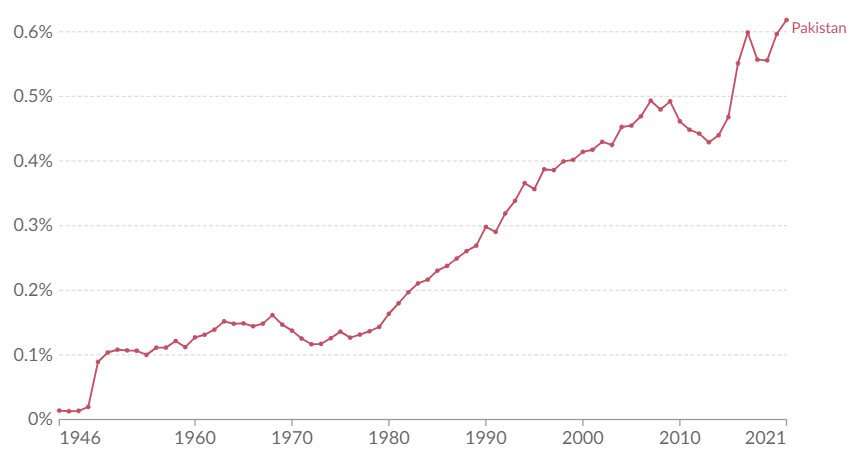
\includegraphics[width=0.45\textwidth]{annual_share.png}
    \caption{Pakistan's Annual Share of Global $CO_2$ Emissions}
    \label{fig:pak-emissions}
\end{figure}

\subsection{Effects of Global Warming}
Although Pakistan contributes less than 1\% of the total global greenhouse gas
emissions, it is one of the most vulnerable countries to the effects of global
warming and climate change. Pakistan is ranked 8th in the world in terms of
climate change vulnerability according to the Global Climate Risk Index 2020
\cite{Eckstein_Künzel_Schäfer_Winges}. The country is already experiencing the
effects of global warming and climate change, an example being the floods in
Karachi in August 2020. The floods were caused by heavy rainfall, which is a
direct effect of global warming and climate change. A more recent example are
the floods in Sindh in July 2022, which were also caused by heavy rainfall.
These floods have caused extensive damage to property and infrastructure, and
have also resulted in loss of life. The estimated cost of the damage caused by
the floods was as high as \$40bn \cite{Javaid_2022}. These events are not
isolated incidents, and they will continue to occur more frequently as global
warming and climate change worsen.

\subsection{Prevention of Global Warming}
Along with the rest of the world, Pakistan needs to take action to prevent
global warming and climate change. The country needs to reduce its greenhouse
gas emissions by transitioning to renewable energy sources such as solar and
wind power. Pakistan also needs to improve energy efficiency in all sectors of
the economy, including the energy, agriculture, industrial processes, waste,
and land-use sectors. The country also needs to improve its infrastructure to
better withstand the effects of global warming and climate change, such as
floods and droughts.

Pakistan is already taking steps to prevent global warming and climate change.
In it's updated Nationally Determined Contribution (NDC), Pakistan has set a
target of generating 60\% of its electricity from renewable sources by 2030
\cite{UNDP_Climate_Promise}. The country is also pushing for the adoption of
electric vehicles, which will help to reduce greenhouse gas emissions from the
transportation sector. Pakistan intends to reduce its greenhouse gas emissions
by 15\% by 2030 using its own resources, and by 30\% by 2030 with international
support with an overall goal of reducing its emissions by 50\% by 2030
\cite{UNDP_Climate_Promise}.

\section{Conclusion}
Global warming and climate change are very serious issues that need to be
addressed as soon as possible. The effects of global warming and climate change
are already being felt around the world, and they will only get worse if we do
not take action now. The causes of global warming and climate change are
primarily due to human activities, such as the burning of fossil fuels and the
clearing of forests. Renewable energy and energy efficiency are the two most
important ways to prevent global warming and climate change. Pakistan is one of
the most vulnerable countries to the effects of global warming and climate
change, and it needs to work with the rest of the world to prevent global
warming and climate change.

\printbibliography

\end{document}